%--------------------------------------------------------------------------
%
%                                                    SOLUTION
%
%--------------------------------------------------------------------------

\begin{center}
\vspace*{5mm}
\noindent {\Large {\bf (Solution) }}
\end{center}

\begin{enumerate}
\item[a)] To form a direct orthonormal coordinate system $Oxyz$ with the $x$ and $z$ axes, the $y$-axis must be perpendicular to the other two. Therefore, it is perpendicular to the watch face's plane. At 9~am, the $y$-axis points to the back of the watch, while at 3~pm it points to the front.
\hspace*{0.5cm}
\begin{center}
 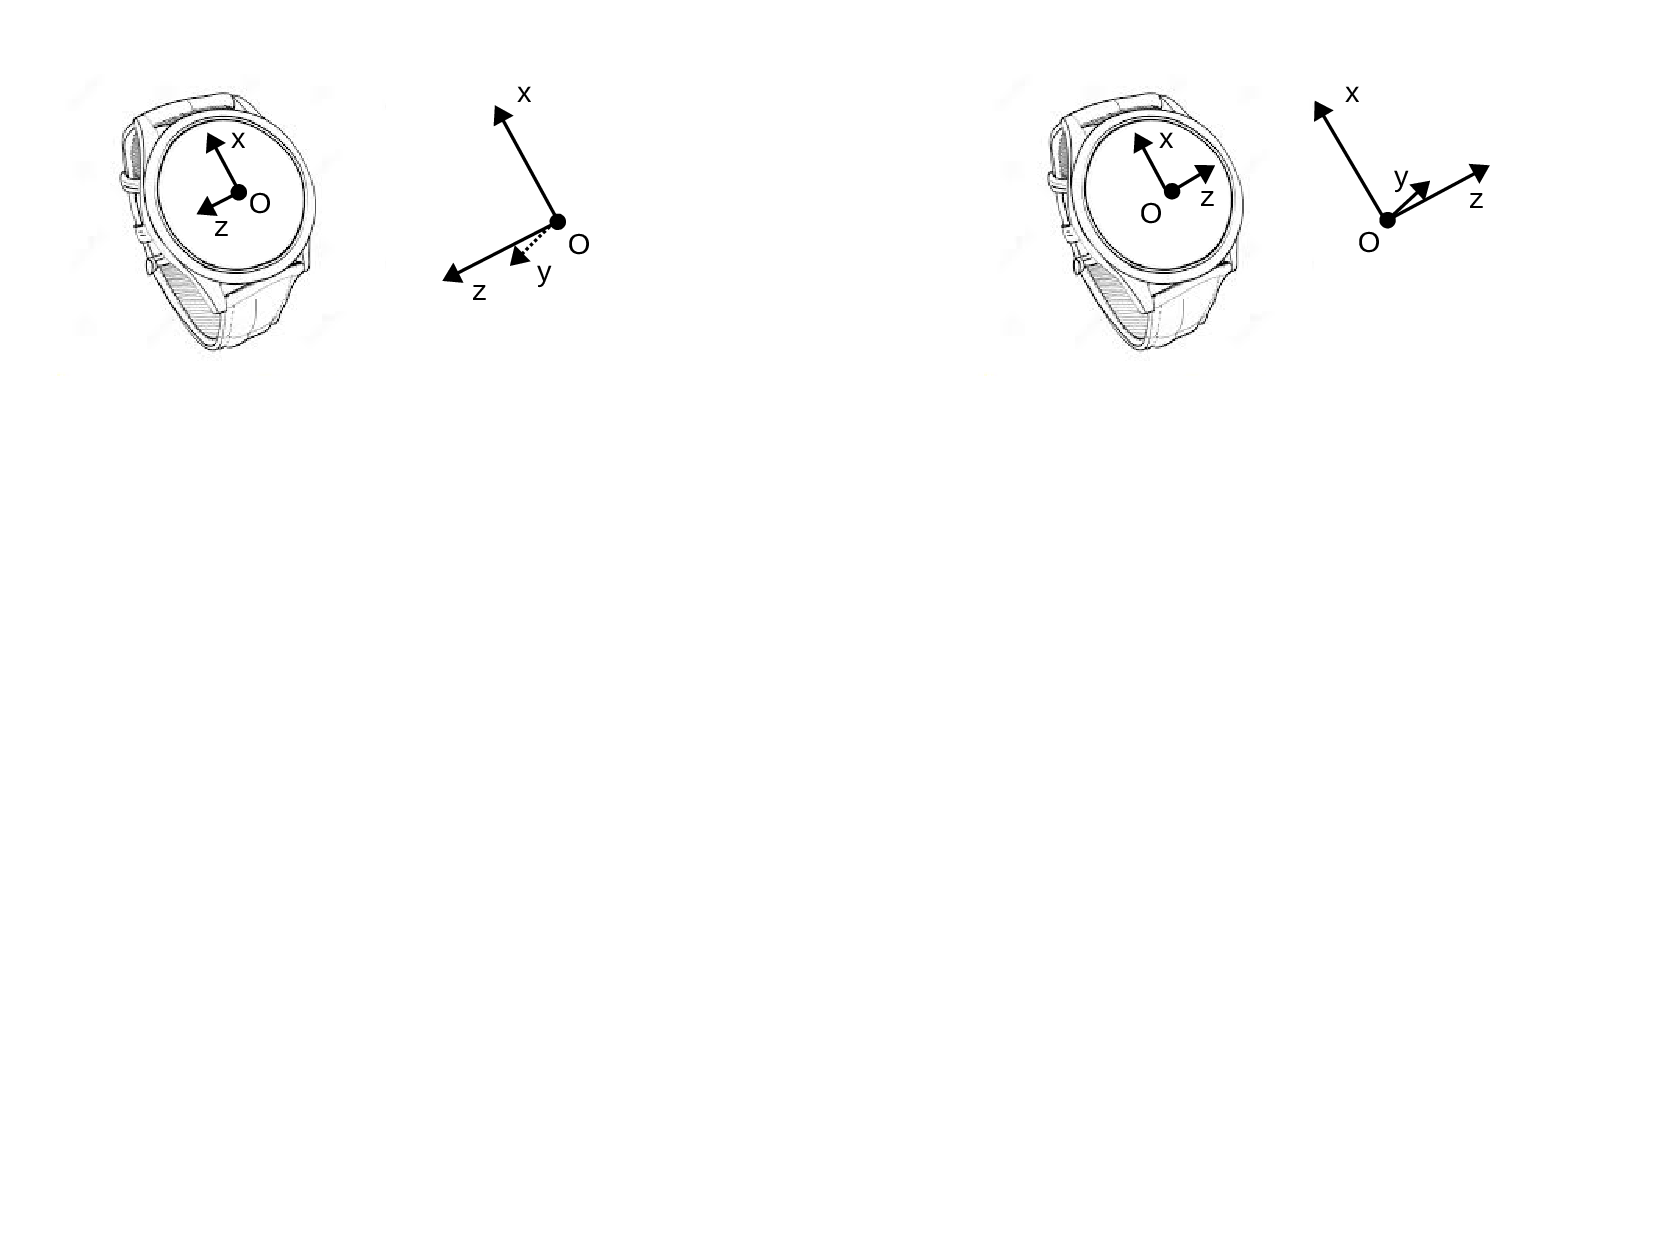
\includegraphics[width=18cm,trim={0 14cm 0cm 0},clip]{figures/Question_Concept_2.pdf}
\end{center}
\end{enumerate}
\begin{minipage}{0.6\textwidth}\begin{enumerate}
\item[b)] Since the sun rises East and sets West, the Earth is rotating from West to East (cf. $\vec{v}$ on the diagram). The angular velocity vector $\vec{\omega}$ is defined such that: $\vec{v}=\vec{\omega}\wedge\vec{r}$. $\vec{\omega}$ is parallel to the Earth's rotational axis, and its direction is the Earth's direction of rotation. Using the right-hand rule, we find that the angular velocity vector must be directed from the South Pole to the North Pole.
\end{enumerate}
\end{minipage}
\begin{minipage}{0.4\textwidth}\begin{center}
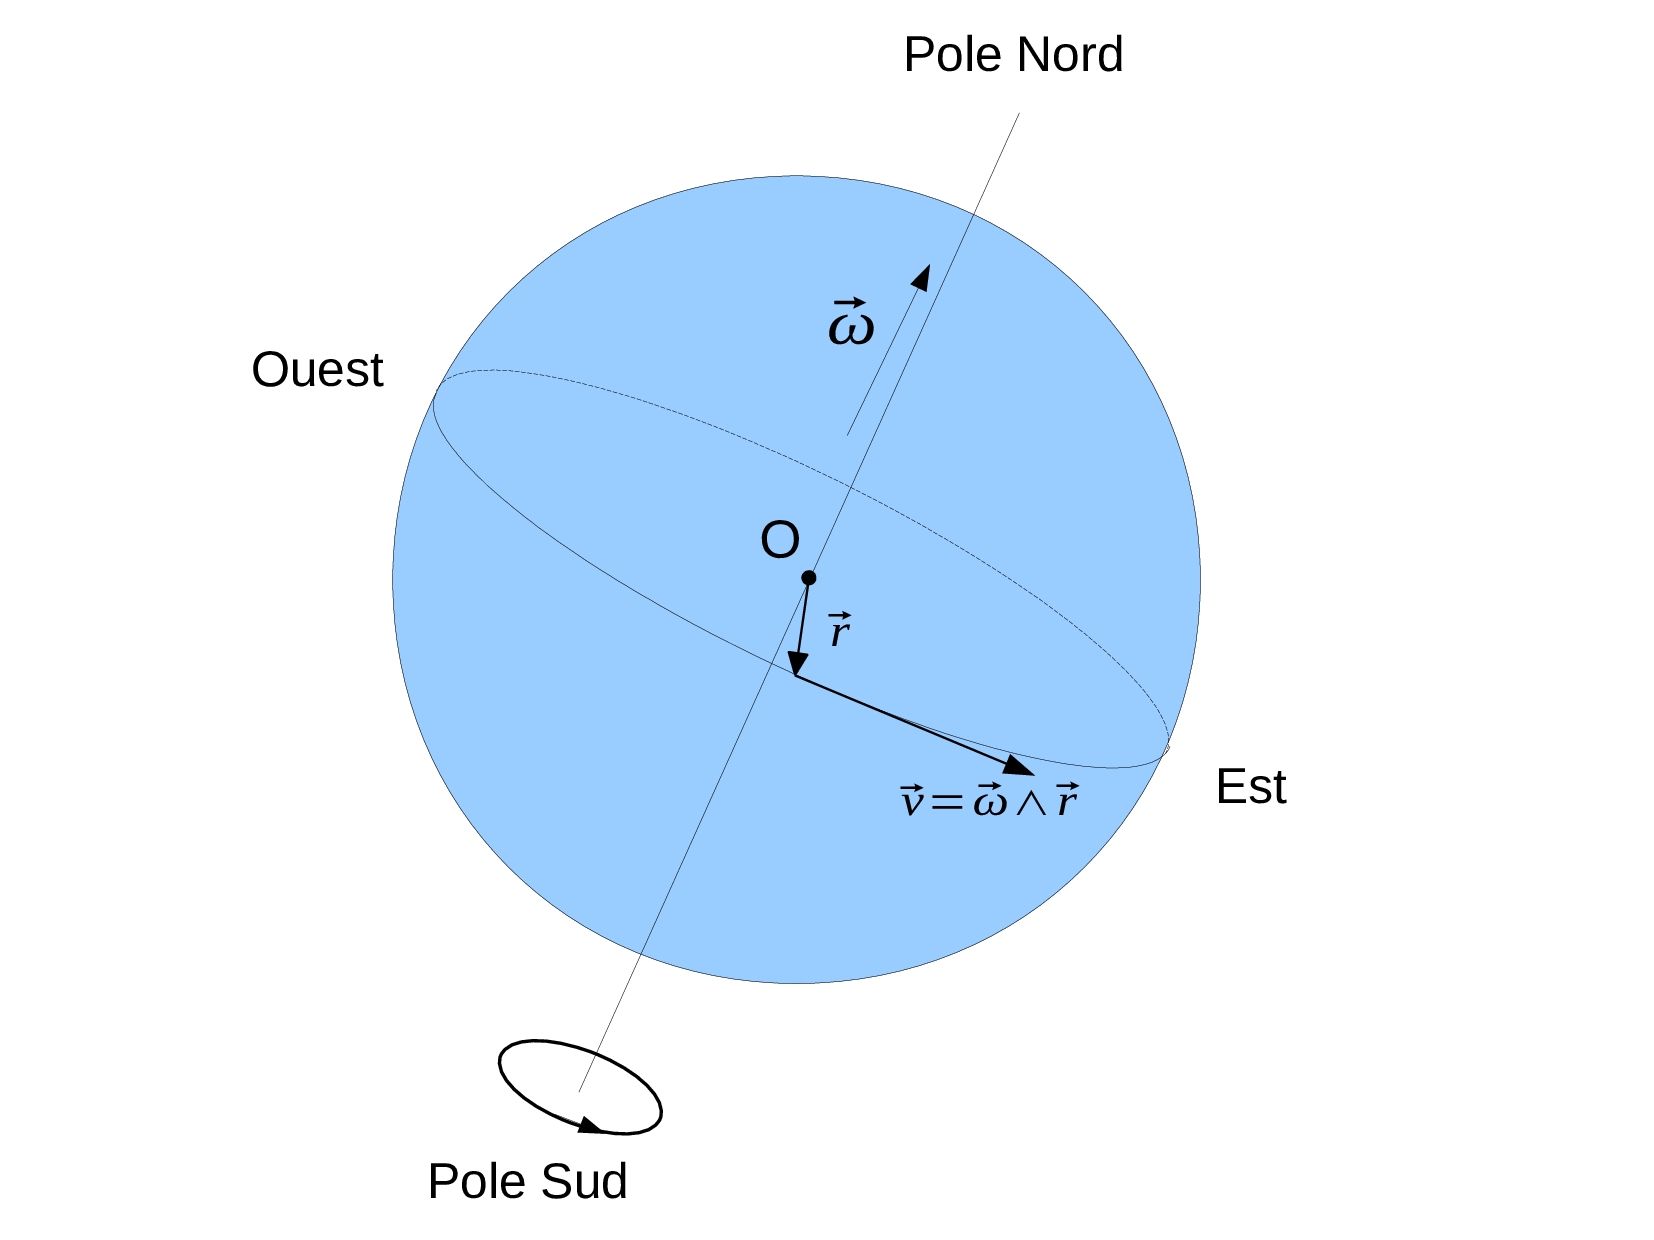
\includegraphics[scale=0.3]{figures/Question_Concept_3.pdf}
\end{center}
\end{minipage}
